\chapter{Evaluation}

The main problem of the current implementation in Bdrive is the scalability of the file keys. For each new device, a new file key needs to be created and maintained. The proposed prototype servers as the proof of concept that such a distributed secure system can exist that fit all the requirements of section \req{sec:requirements} and scale better than the current system implemented in Bdrive regarding the number of file keys. 

To stress this last point, different benchmarks will be conducted to compare the proposed prototype to a similar environment such as Bdrive. The goal of this section will be to show that the assumption following assumption holds true:

\begin{center}
\textit{The ABE-based solution, of the in section \ref{sec:implementation} proposed system to solve the scalability problem of a secure cloud storage system, scales at least as good as the RSA-based approach, described in section \ref{sec:background}, regarding the number of file keys that need to be maintained.}
\end{center}

While this assumption should hold true on group operations such as member join and file upload, the proposed approach comes with an additional overhead on member removal due to additional shared-key revocation management. 

\section{Upper-Bound and Worst-Case Scenario}
In this section it will theoretically argued why \name scales at least as good as the current solution for secure cloud storage systems. The number of files keys per $n$ user scale with $O(n)$ (same way as Bdrive) in \name if and only if, no suitable subset of district attributes of any two users can be found so that the $n$ users can be described with $a < n$ attributes $a$. 
That means that if in that group at least two users would share the same attribute only $a < n$ attributes would be needed to describe this group, resulting in $a$ file keys. 
If that is not the case, say no user share the same attribute, for each user an unique attribute needs to be used (for example the email address of the user) which is embedded in an inclusive attribute policy. 

\begin{center}
\begin{lstlisting}[caption={Worst case access policy. The used email address is a unique attribute per user.},captionpos=b]
(alice@example.com OR bob@example.com OR ... OR zara@example.com)
\end{lstlisting}
\end{center}

Such policy will spawn each unique attribute of the users combining them with an "OR" (see above example). As described in section \ref{sec:extension-to-dnf-policy} this will case the creation of $n$ cipher texts, the exact same number of file keys that will also be created in Bdrive. 

The remaining assumption that needs to be shown is that for each "AND" used in the access policy the resulting number of cipher text will be effective smaller then the number of users. 

\section{Performance and Scalability Analysis}


\section{Future adaptations}

\todo{
* Data owner Id can relate to the selected two factor key. 
* This would enable us to have multible keys 2FA keys per user. each securing an own CT. 
* make ownerId -> 2FA id 

* Handle attributes on device level and not on user level 
}

\section{Conclusion}
\begin{figure}[!t]
\centering
    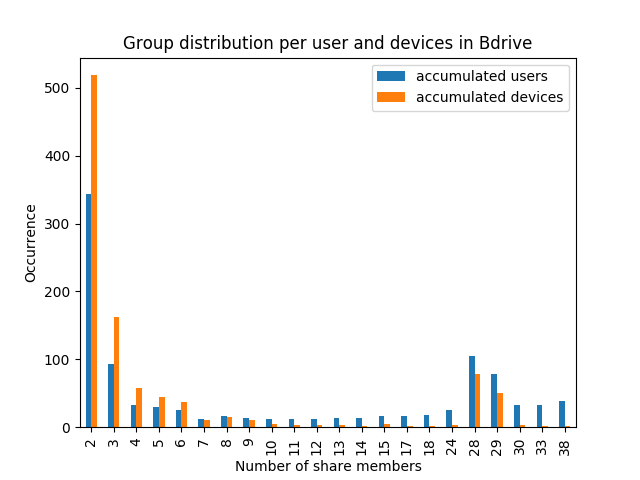
\includegraphics[width=1.0\linewidth]{img/share_distribution_bdirve.png}
    \caption{The distribution of shared folders per users and their aggregated devices.}
    \label{fig:evaluation-share-distribution}
\end{figure}
